\subsection{Dashboard}\label{subsec:dashboard2}

The \textbf{Dashboard screen} is immediately after the \textbf{Splash screen}.
We is counted on the fact a user will spend most of the time on the \textbf{Dashboard screen}, and so it contains the of the functionalities.
This screen is divided into:
\begin{itemize}
    \item Top panel,
    \item Map controls and
    \item Fly now button.
\end{itemize}
These elements are in the higher stack layer below the map where are placed flying drones, place pins and restricted areas.
Besides, it allows displaying without wasteful \textbf{POIs} (Point of Interest)\cite{poi}, satellite map or standard map, which contains POIs, precisely like \textbf{Google Maps} application.

The Top panel is consists of:
\begin{itemize}
    \item Device status - it contains current information about default device,
    \item Search button - it is for searching of places, devices, aircrafts and zones and
    \item Profile button - it represents the main menu of the whole application.
\end{itemize}
If a user has already logged in and planned a flight, Profile button contains a light blue circle with the number of planned flights in the top right on the circuit of that circle button.
The key difference we can see on the picture~\ref{fig:dashboard}.

Map controls are consists of:
\begin{itemize}
    \item My location button - it redirects to his position due to his location by GPS coordinates,
    \item Map layers button - it is an offer allowing us to choose a map style and
    \item Fly now button - this button disappears options Fly now and Plan a flight for already logged in user and Log in and sign up button for an unauthorized user.
\end{itemize}
These are additional elements showing on the \textbf{Dashboard screen}:
\begin{itemize}
    \item Drone detail panel, (Figure \ref{fig:dashboard_drone_detail})
    \item Place detail panel,
    \item Zone detail panel, (Figure \ref{fig:dashboard_zone_detail})
    \item Zone selection panel, and
    \item Map layer panel.
\end{itemize}

The \textbf{Drone detail panel} is for showing necessary information and a flying drone and its flight parameters.
Besides, it contains the button to redirection to the full drone detail screen, where a user can see all information about live flight immediately.

The \textbf{Place detail panel} contains necessary information about the place.
Also, if a user wants to plan a flight from this place, it allows us to pin this place until the user unpins it from the map and Plan a flight button.
Place pinning into the map is demonstrated by a color change of the pin and color change of the icon in the panel.

The \textbf{Zone detail panel} contains necessary information about the given zone, such as a lower altitude level, upper altitude level, name of the zone, and validation from and zone status.

The \textbf{Zone selection} is used to select a zone if a user clicks to a place in the map where is an intersection of more zones.
Simultaneously, when this selection is shown, the selected zones are highlighted.
If a user chooses a zone, the zone will show Zone detail panel and will highlight only one particular zone instead of the intersection.

We focused on the primary purpose of informing a user about drones and restricted areas around him.
So, we decided to keep a minimalistic design because the user needs to emphasize what is important to him.


\begin{figure}
    \centering
    \begin{minipage}{.4\textwidth}
        \centering
        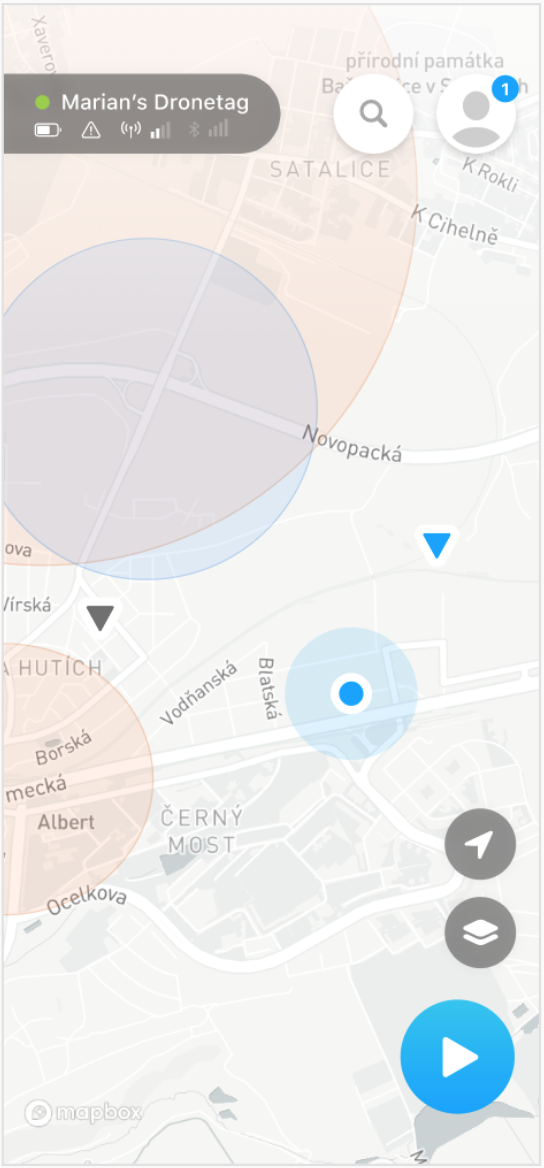
\includegraphics[width=.7\linewidth]{assets/user_interface_design/dashboard/dashboard.png}
        \caption{Dashboard}
        \label{fig:dashboard}
    \end{minipage}%
    \hspace{.05\linewidth}
    \begin{minipage}{.4\textwidth}
        \centering
        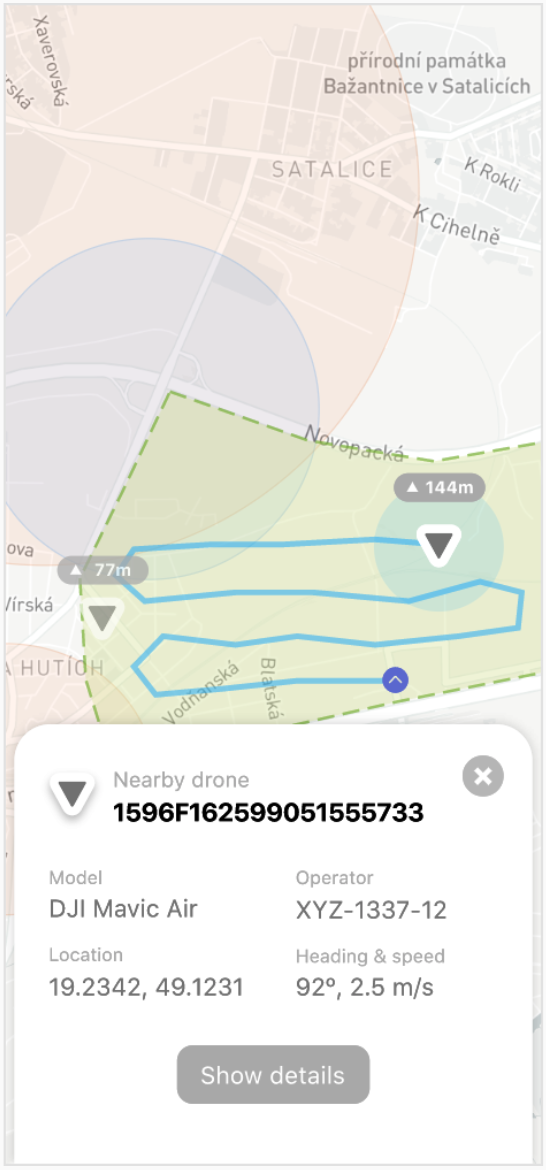
\includegraphics[width=.7\linewidth]{assets/user_interface_design/dashboard/dashboard_drone_detail.png}
        \caption{Dashboard, Drone detail}
        \label{fig:dashboard_drone_detail}
    \end{minipage}
    \label{fig:dashboard_all}
\end{figure}
